\documentclass[a4paper,10pt,oneside]{article}
\usepackage[polutonikogreek,italian]{babel}
\usepackage[utf8x]{inputenc}
\usepackage{amsmath}
\usepackage{amsthm}
\usepackage{amssymb}
\usepackage{amscd}
\usepackage{graphicx}
\usepackage{float}
\usepackage{array}
\usepackage{rotating}
\usepackage[small]{caption}
\usepackage{lscape}
\usepackage{fancybox}
\usepackage{booktabs}
\usepackage[noanswer]{exercise}
\parindent0ex
\renewcommand{\fboxsep}{0.4cm}
\usepackage{hyperref}
\renewcommand{\textfraction}{0.05}
\renewcommand{\topfraction}{0.95}
\renewcommand{\bottomfraction}{0.95}
\renewcommand{\floatpagefraction}{0.35}
\renewcommand{\ExerciseName}{Esercizio}
\renewcommand{\ExerciseListName}{Es}
\setcounter{totalnumber}{5}
\restylefloat{figure}
\begin{document}
\thispagestyle{empty}
\section*{Conservazione della quantità di moto}

\vspace{4cm}

Ricaviamo la legge di conservazione della quantità di moto supponendo che le forze in gioco nel sistema siano di tipo newtoniano, ovvero che in ogni istante valga la relazione $\mathbf{F}_{12}=-\mathbf{F}_{21}$.
Ricordando che la quantità di moto (nel caso non relativistico) è definita come:
\begin{equation}
 \mathbf{p}=m\mathbf{v}
\end{equation}
possiamo scrivere la prima legge di Newton in forma più generale come:
\begin{equation}
 \mathbf{F}=\frac{d\mathbf{p}}{dt}
\end{equation}
che si riduce alla forma elementare della prima legge della meccanica nel caso in cui la massa sia costante.
Per ricavare la legge di conservazione della quantità di moto applichiamo il terzo principio della dinamica a due corpi in interazione (ad esempio due sfere che collidono) per un determinato intervallo di tempo finito $\Delta t$, le forze risultanti saranno:
\begin{equation}
 \mathbf{F}_{12}=M_1\frac{\Delta \mathbf{v}_1}{\Delta t}
\end{equation}
e
\begin{equation}
 \mathbf{F}_{21}=M_2\frac{\Delta \mathbf{v}_2}{\Delta t}
\end{equation}
per il terzo principio possiamo scrivere:
\begin{equation}\label{terzo}
 M_1\frac{\Delta \mathbf{v}_1}{\Delta t}=-M_2\frac{\Delta \mathbf{v}_2}{\Delta t}
\end{equation}
La relazione [\ref{terzo}] deve valere per ogni intervallo di tempo $\Delta t$, questo ci permette di scrivere:
\begin{equation}\label{princ}
 (M_1\mathbf{v}_1+M_2\mathbf{v}_2)_{iniziale}=(M_1\mathbf{v}_1+M_2\mathbf{v}_2)_{finale}
\end{equation}
La [\ref{princ}] vale chiaramente,istante per istante, solo supponendo che le forze si propaghino con velocità infinita\footnote{Ovvero nell'ipotesi di forze newtoniane}.

\section*{Urti unidimensionali}

Applichiamo ora la conservazione della quantità di moto al caso semplice degli urti unidimensionali. Teoricamente possiamo distinguere due casi estremi:
\begin{itemize}
 \item Gli urti perfettamente elastici
 \item Gli urti totalmente anaelastici
\end{itemize}
Nel primo l'energia cinetica totale si conserva mentre non lo fa  nel secondo, in laboratorio osserveremo dei casi intermedi ovvero l'energia cinetica ne si conserverà completamente ne si dissiperà massimamente.

Il caso unidimensionale si può studiare ed analizzare utilizzando solo la conservazione dell'energia e della quantità di moto. Facendo riferimento a quanto vedremo in laboratorio, consideriamo due carrelli di masse $m$ ed $M$ liberi di scivolare, quasi senza attrito, lungo la guidovia a cuscino d'aria. Consideriamo inizialmente il caso elastico, possiamo scrivere il sistema:
\begin{equation}\label{urti_1}
 \begin{cases}
  mv_1+Mv_2=mu_1+Mu_2\\
  \frac 1 2 mv_1^2+\frac 1 2 Mv_2^2=\frac 1 2 mu_1^2+\frac 1 2 M u_2^2
 \end{cases}
\end{equation}
dove abbiamo imposto la conservazione dell'energia e della quantità di moto, le $u_1$ e $u_2$ sono le velocità dei due carrelli dopo l'urto.
Riscriviamo ora la conservazione dell'energia portando gli addendi contenenti velocità dello stesso carrello nello stesso membro:
\begin{equation}
 mv_1^2-mu_1^2=Mu_2^2-Mv_2^2
\end{equation}
raccogliamo le masse e applichiamo una nota proprietà algebrica:
\begin{equation}\label{energ_1}
 m(v_1+u_1)(v_1-u_1)=M(u_2+v_2)(u_2-v_2)
\end{equation}
Riscriviamo ora la legge di conservazione della quantità di moto portando i termini che si riferiscono allo stesso carrello nello stesso membro:
\begin{equation}
 mv_1-mu_1=Mu_2-Mv_2
\end{equation}
raccogliendo le masse:
\begin{equation}\label{qm_1}
 m(v_1-mu_1)=M(u_2-v_2)
\end{equation}
Confrontiamo ora l'equazione [\ref{energ_1}] con la [\ref{qm_1}], otteniamo la relazione:
\begin{equation}
 v_1+u_1=u_2+v_2
\end{equation}
che può essere riscritta come:
\begin{equation}\label{newton1}
 v_1-v_2=-(u_1-u_2)
\end{equation}
la relazione [\ref{newton1}] ci dice che le velocità relative dei due carrelli prima dell'urto e dopo l'urto sono opposte.
Se ora riscriviamo la [\ref{urti_1}] utilizzando la [\ref{newton1}] in vece della legge di conservazione dell'energia otteniamo il sistema \footnote{Nel caso unidimensionale è assolutamente equivalente risolvere l'uno o l'altro sistema}
\begin{equation}
 \begin{cases}
  v_1-v_2=-(u_1-u_2)\\
  mv_1+Mv_2=mu_1+Mu_2\\
 \end{cases}
\end{equation}
risolvendo il sistema otteniamo per le due velocità:
\begin{equation}
 \begin{cases}
    u_1=\dfrac{(m-M)v_1+2Mv_2}{m+M}\\
\\
    u_2=\dfrac{(M-m)v_2+2Mv_1}{m+M}
 \end{cases}
\end{equation}
In laboratorio simuleremo un urto quasi elastico facendo scontrare i due carrelli della guidovia fra cui avremo frapposto una molla.
Per trattare i casi reali parzialmente anaelastici introduciamo il coefficiente di restituzione $\epsilon$ cui assegniamo valore 1 nel caso in cui l'urto sia perfettamente elastico e il valore 0 nel caso in cui l'urto sia totalmente anaelastico. Inserendo questa quantità nella [\ref{newton1}] otteniamo la relazione:
\begin{equation}\label{newton2}
 v_1-v_2=-\epsilon(u_1-u_2)
\end{equation}
conosciuta come regola dell'urto di Newton. Se ora risolviamo il sistema più generale:
\begin{equation}
 \begin{cases}
  v_1-v_2=-\epsilon(u_1-u_2)\\
  mv_1+Mv_2=mu_1+Mu_2\\
 \end{cases}
\end{equation}

otteniamo il risultato:
\begin{equation}\label{unid_eps}
 \begin{cases}
    u_1=\dfrac{(\epsilon m-M)v_1+(1+\epsilon)Mv_2}{m+M}\\
\\
    u_2=\dfrac{(\epsilon M-m)v_2+(1+\epsilon)Mv_1}{m+M}
 \end{cases}
\end{equation}
in un urto unidimensionale reale le velocità dopo l'urto saranno sempre date dalla [\ref{unid_eps}].

In laboratorio simuleremo un urto anaelastico  utilizzando sostanze collose in modo che i carrelli tendano ad aderire.

\subsection*{Misura della velocità di uscita dell'acqua dall'ugello di una siringa}

In questa esperienza utilizzeremo la legge di conservazione della quantità di moto per stimare la velocità media di uscita dell'acqua dall'ugello di una siringa. Il carrello di massa complessiva (con imbuto e raccoglitore dell'acqua) $M_1$ viene colpito dal getto d'acqua della siringa e inizia a muoversi lungo la guidovia. La legge di conservazione in esame ci assicura che la quantità di moto totale dell'acqua lungo l'asse orizzontale si trasferisce al carrello,  per cui se questo è inizialmente fermo possiamo scrivere

\begin{equation}
M_av_{i}=(M_1+M_a)v_f
\end{equation}
se il carrello ha invece una velocità iniziale non nulla 
\begin{equation}
 M_1v_{i_{carrello}}+M_av_{i_{ugello}}=(M_1+M_a)v_f
\end{equation}
dove con $M_a$ abbiamo indicato la massa totale dell'acqua.


\begin{figure}[H]
 \centering
 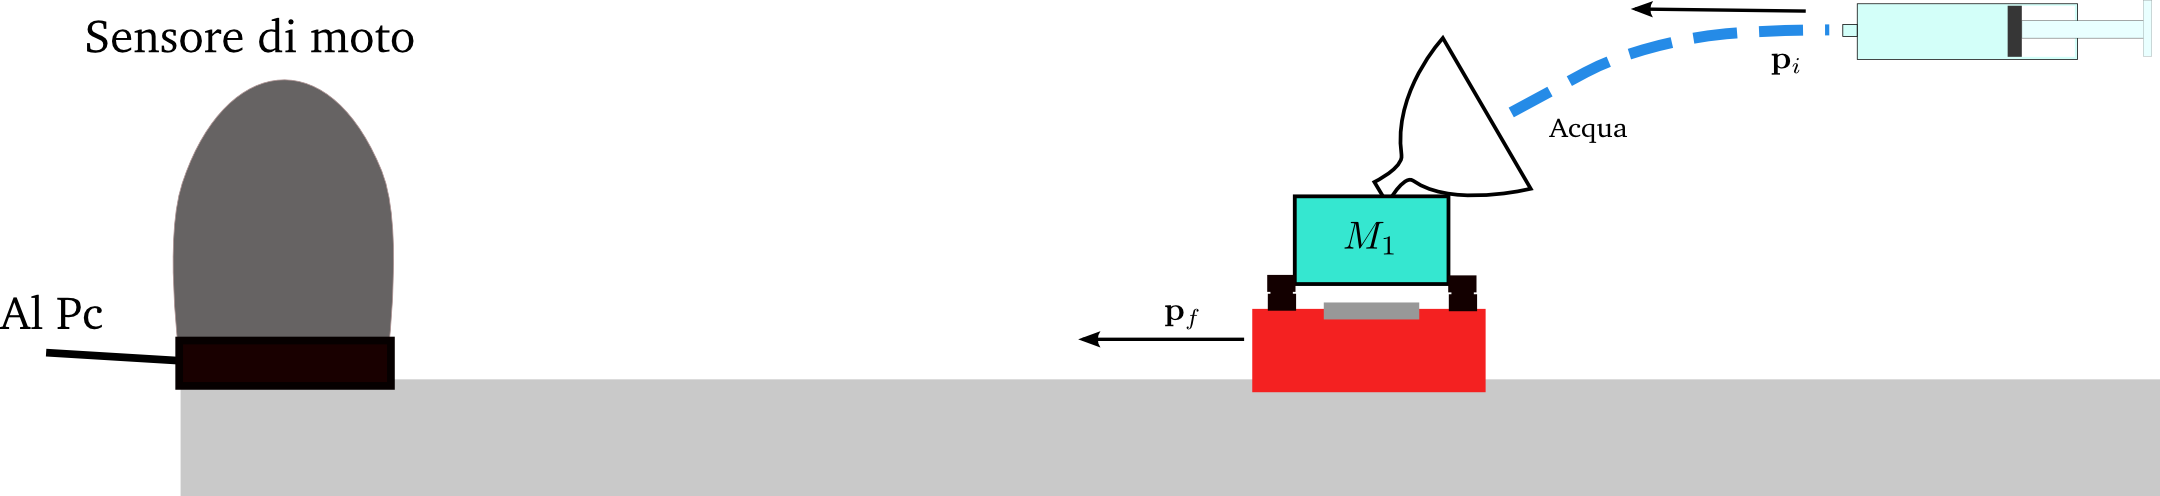
\includegraphics[width=\textwidth]{./immagini/imbuto.png}
 % imbuto.png: 2160x496 pixel, 300dpi, 18.29x4.20 cm, bb=0 0 518 119
 \caption{Determinazione della componente $x$ della quantità di moto dell'acqua in uscita dalla siringa}
 \label{fig:imbuto_siringa}
\end{figure}
misurando la velocità finale $v_f$ del carrello caricato dell'acqua emessa dalla siringa possiamo dedurre la velocità iniziale (media) dell'acqua in uscita dall'ugello:
\begin{equation}
 v_i=\frac{M_1+M_a}{M_a}v_f
\end{equation}

\section*{Urti bidimensionali}

Negli urti in due o più dimensioni la legge di conservazione dell'energia e la legge di conservazione della quantità di moto non sono più sufficienti per determinare le velocità finali a partire da quelle iniziali, in generale sarà necessario introdurre delle informazioni riguardo il tipo di interazione e la geometria degli oggetti coinvolti. In questo laboratorio  ci limiteremo ad analizzare, matematicamente, il caso di sfere perfette e assumeremo valida la legge empirica dell'urto di Newton per le componenti radiali delle velocità delle due sfere, inoltre, per semplificare ulteriormente i calcoli si supporrà inizialmente immobile una delle due sfere. Analizziamo la figura [\ref{fig:sfere diverse}]. Inizialmente solo la sfera $m$ è in moto con velocità $\mathbf{v}_1$, il sistema di riferimento in figura è determinato dalla retta tangente alle due sfere nel punto di impatto e dalla normale a questa passante per i centri delle stesse. La velocità iniziale della sfera $m$ forma un angolo $\theta$ con la direzione tangenziale $\hat{\mathbf{t}}$. Supporremo, inoltre, che sia $m\leq M$.

\begin{figure}[h]
 \centering
 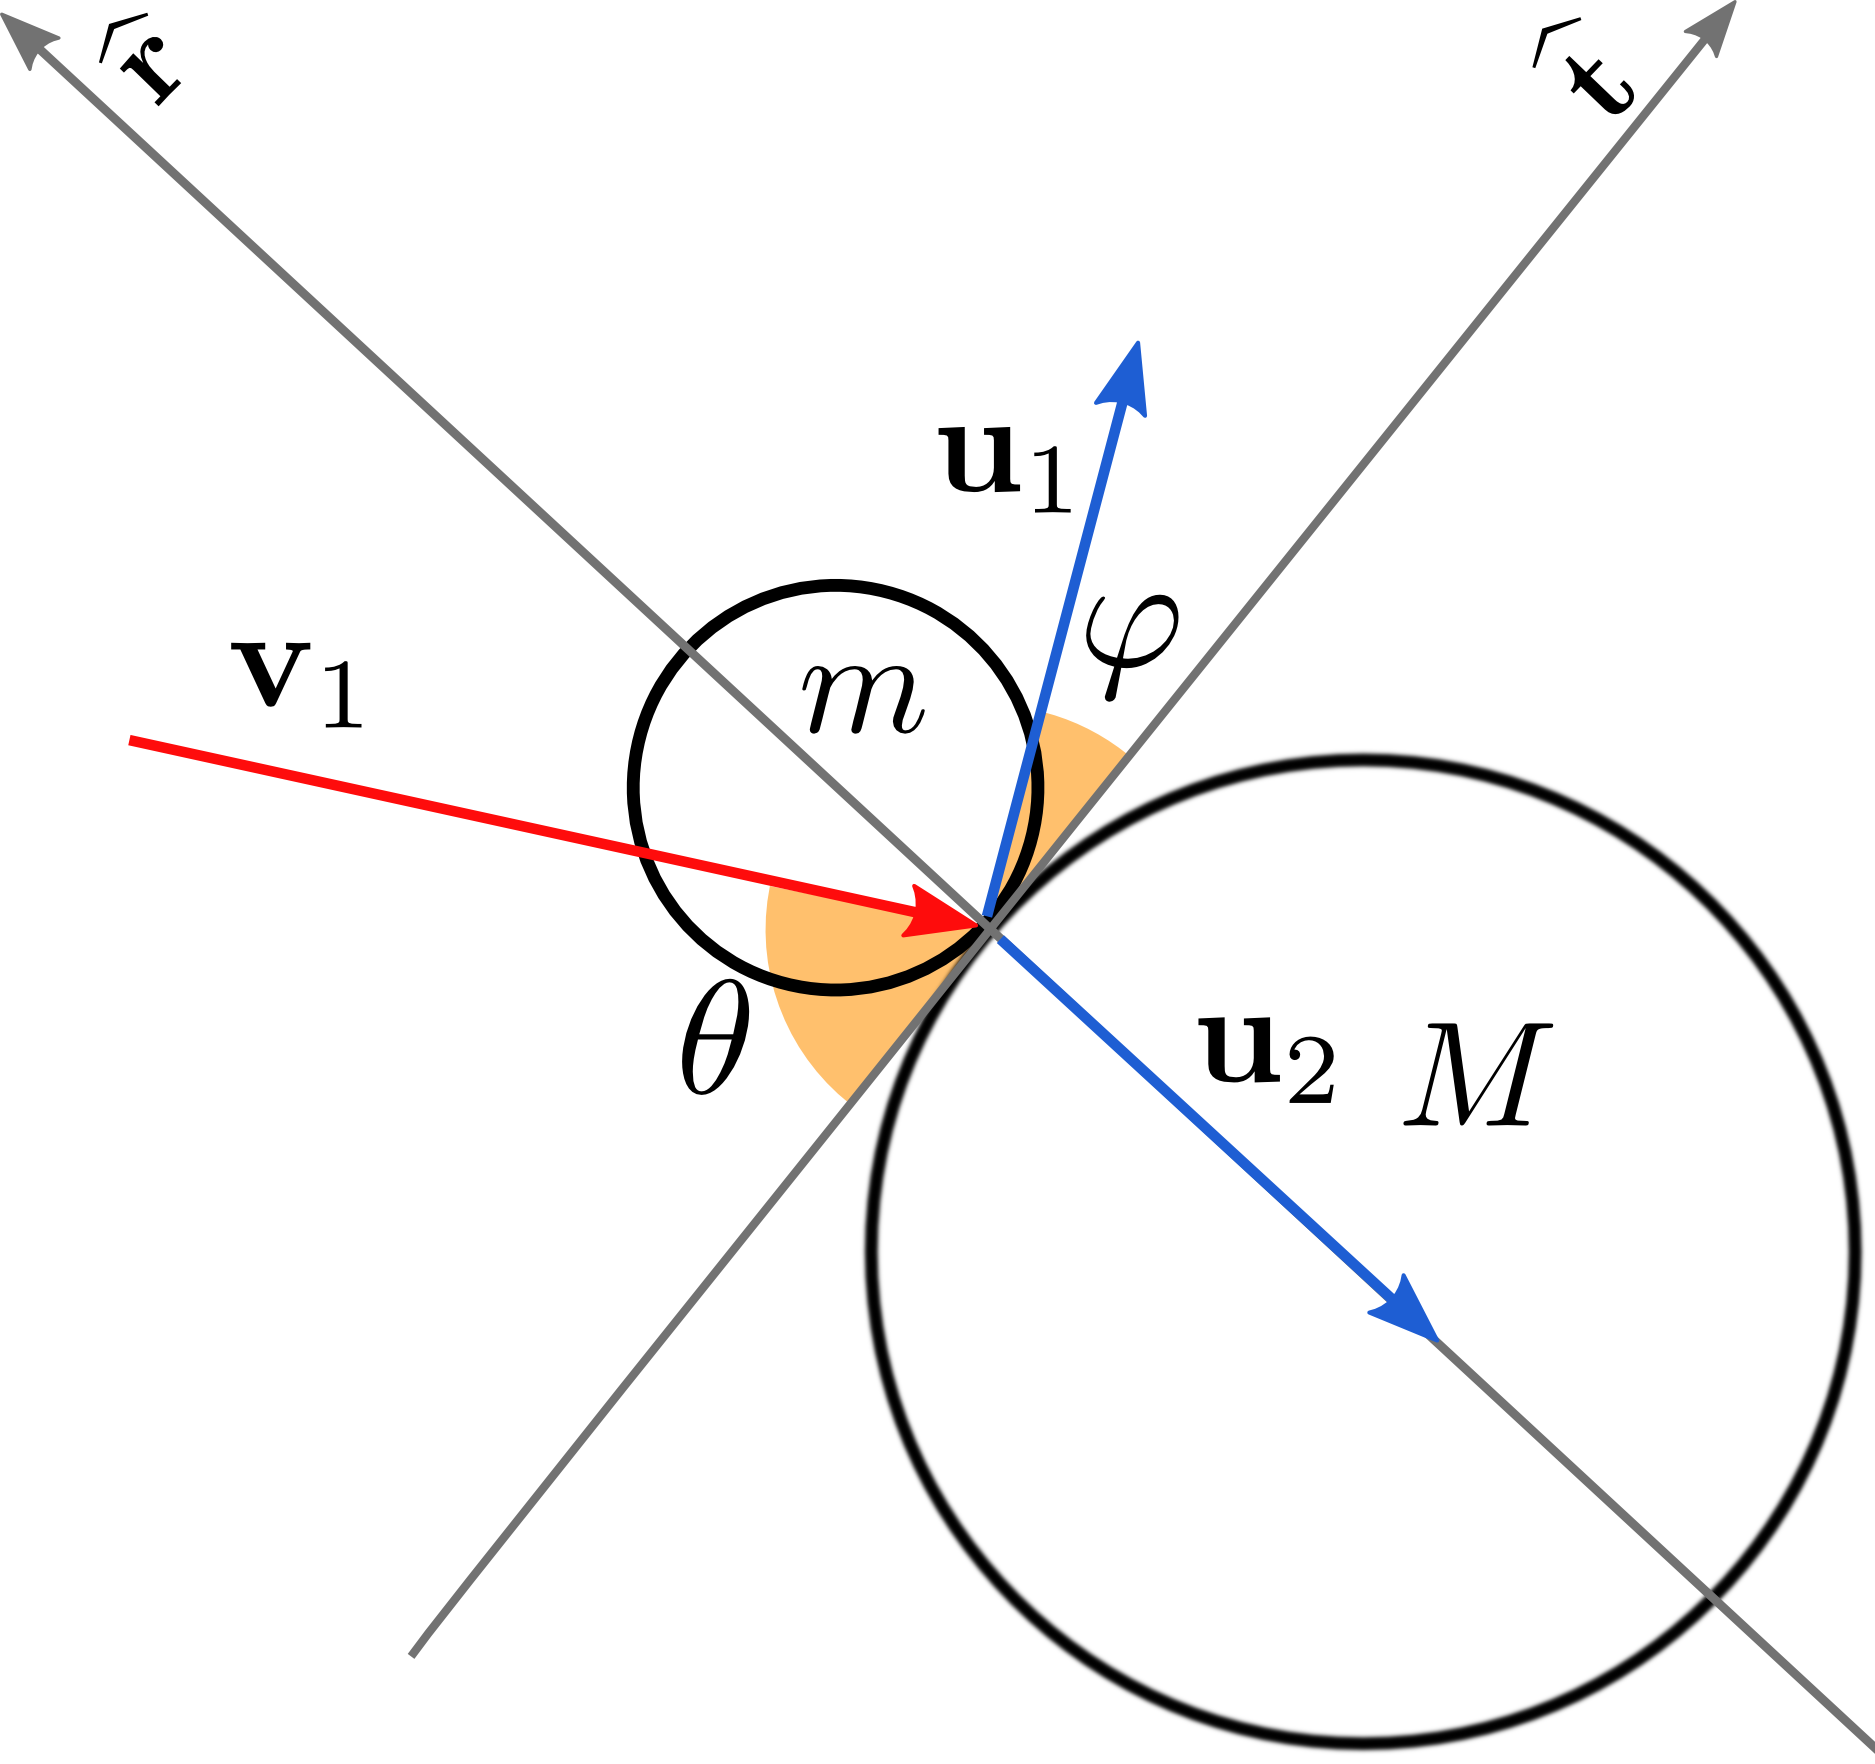
\includegraphics[width=0.6\textwidth]{./immagini/sfere_diverse.png}
 % sfere_diverse.png: 1875x1764 pixel, 500dpi, 9.53x8.96 cm, bb=0 0 270 254
 \caption{La  sfera di massa $M$ è inizialmente immobile, la forza di interazione tra le due sfere si esprime unicamente nella direzione radiale, la velocità tangenziale della sfera di massa $m$ non viene modificata durante l'urto}\label{fig:sfere diverse}
\end{figure}
Scomponendo l'unica velocità iniziale lungo gli assi del nostro sistema di riferimento otteniamo:
\begin{equation}\label{v_iniziale_bi}
 \mathbf{v}_1=(v_1\cos \theta,-v_1\sin\theta)
\end{equation}
dove $v_1$ rappresenta il modulo della velocità. La nostra ipotesi di sfere perfette ci permette di concludere che la forza di interazione tra le due sfere durante l'urto si può esercitare unicamente nella direzione radiale per cui le velocità tangenziali prima e dopo l'urto non dovranno variare:
\begin{equation}
 v_1\cos\theta=u_1\cos\varphi
\end{equation}
dove $u_1$ è il modulo della velocità della sfera $m$ dopo l'urto e $\varphi$ l'angolo che questo forma con la direzione tangenziale.
Per la sfera $M$ sarà invece:
\begin{equation}
 \mathbf{v}_2\cdot\hat{\mathbf{t}}=\mathbf{u}_2\cdot\hat{\mathbf{t}}=0
\end{equation}
dato che inizialmente la sfera $M$ è immobile, la sua velocità finale sarà diretta unicamente lungo la direzione radiale $\hat{\mathbf{r}}$. Per cui siamo in grado di scrivere per $\mathbf{u}_2$:
\begin{equation}
 \mathbf{u}_2=(0,-u_2)
\end{equation}
dove $u_2$ è il modulo di $\mathbf{u}_2$.

\begin{figure}[h]
 \centering
 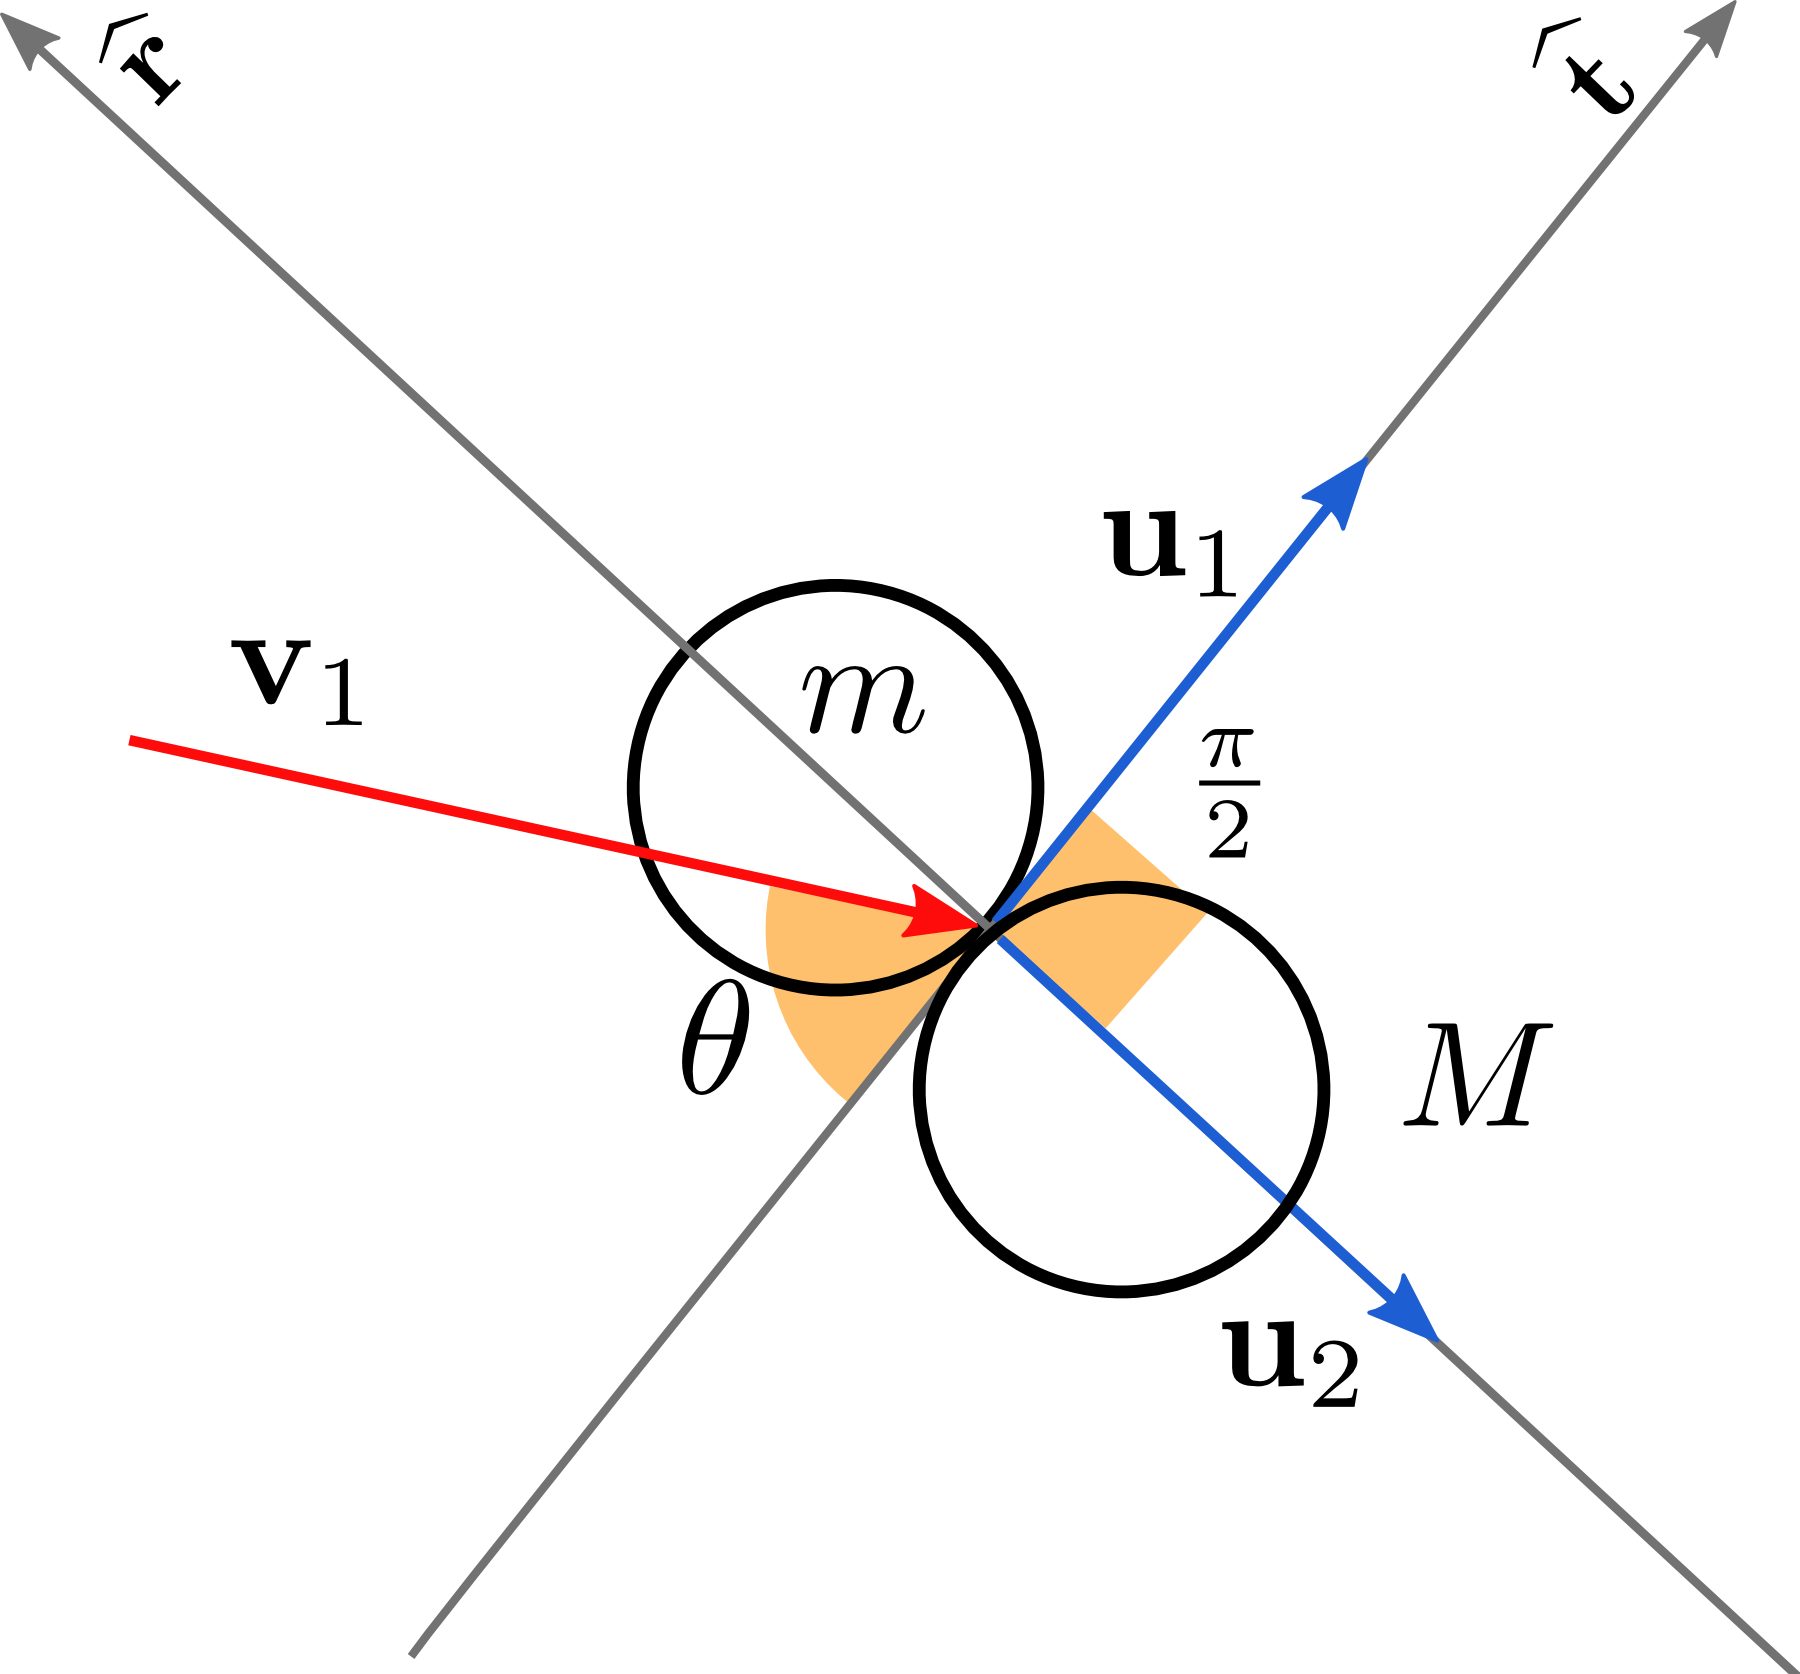
\includegraphics[width=0.6\textwidth]{./immagini/sfere_uguali.png}
 % sfere_uguali.png: 1800x1674 pixel, 500dpi, 9.15x8.51 cm, bb=0 0 259 241
 \caption{Se le masse $m$ ed $M$ delle sfere sono uguali dopo l'urto le loro velocità risultano perpendicolari}\label{fig:sfere_uguali}
\end{figure}
La regola dell'urto di Newton ci dice che la velocità relativa prima dell'urto nella direzione radiale è opposta alla velocità relativa nella stessa direzione dopo l'urto e moltiplicata per un coefficiente di restituzione $\epsilon$. Nel nostro caso semplificato questa legge empirica si traduce in:
\begin{equation} \label{newton_3}
 \mathbf{v}_1\cdot\hat{\mathbf{r}}=-\epsilon(\mathbf{u}_1\cdot\hat{\mathbf{r}}-\mathbf{u_2}\cdot\hat{\mathbf{r}})
\end{equation}
sostituendo nella [\ref{newton_3}] le velocità calcolate precedentemente:
\begin{equation}
 -v_1\sin\theta=-\epsilon(u_1\sin\varphi+u_2)
\end{equation}

o anche:
\begin{equation}
 v_1\sin\theta=\epsilon(u_1\sin\varphi+u_2)
\end{equation}


\begin{figure}[h]
 \centering
 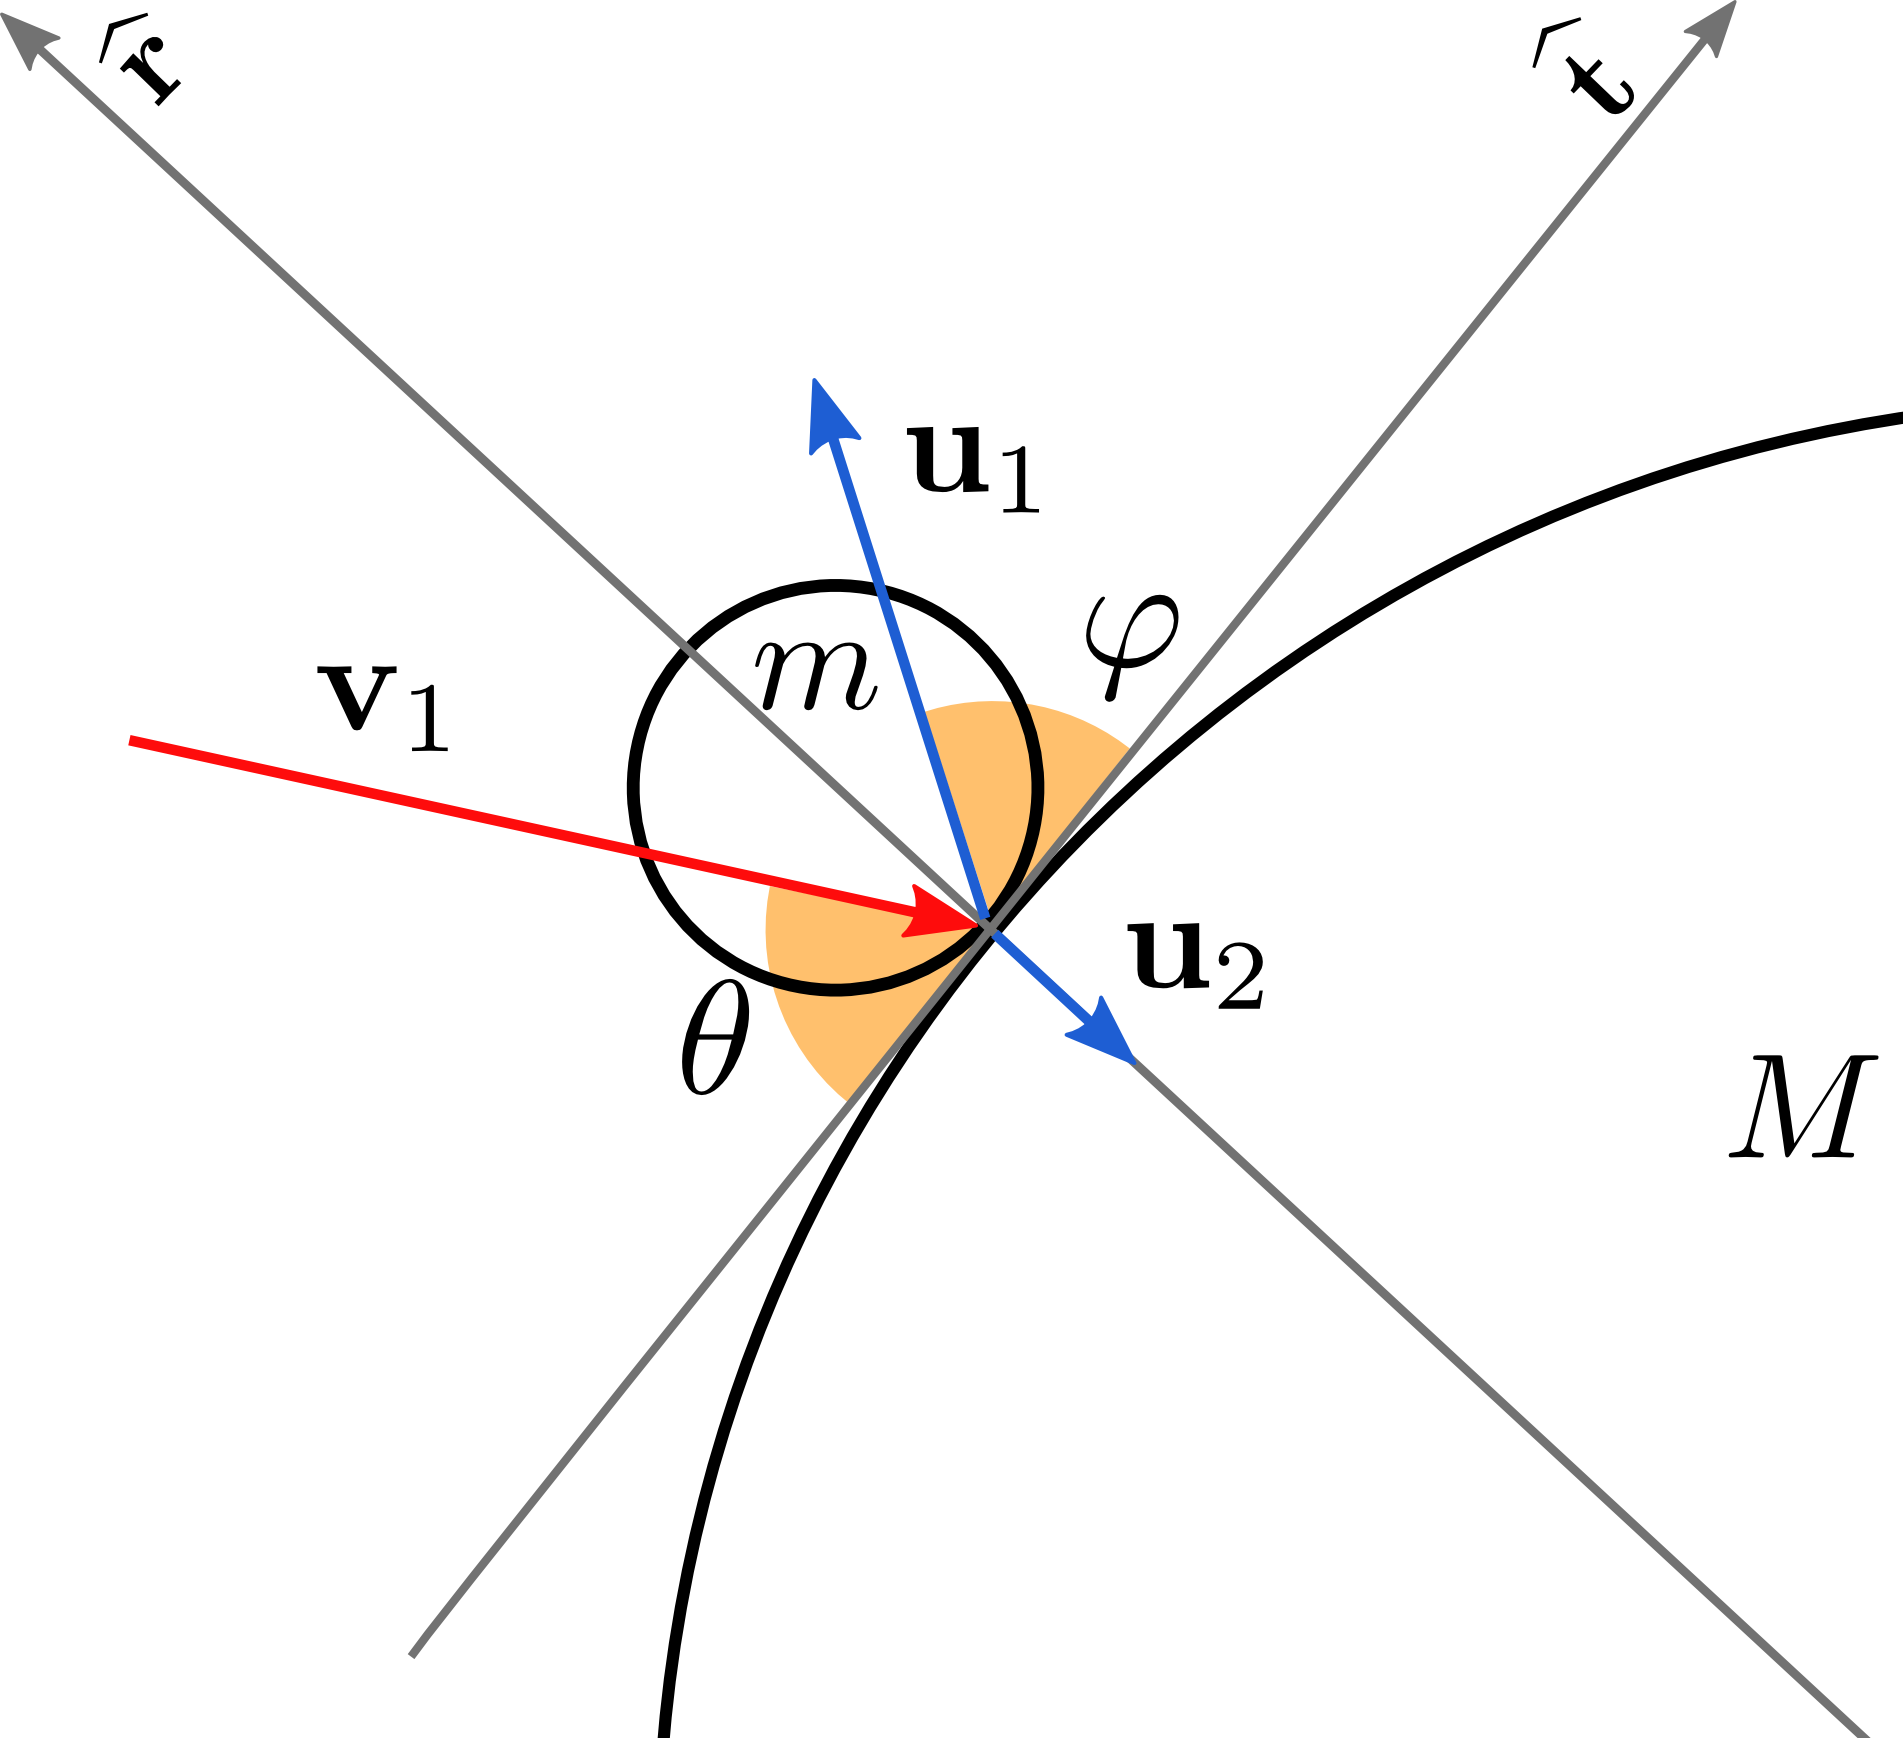
\includegraphics[width=0.6\textwidth]{./immagini/sfere_infinita.png}
 % sfere_infinita.png: 1903x1738 pixel, 500dpi, 9.67x8.83 cm, bb=0 0 274 250
 \caption{Nel limite $M\to\infty$ l'angolo di incidenza $\theta$ e l'angolo di riflessione $\varphi$ risultano uguali, la velocità finale della sfera $M$ è tanto più piccola quanto più grande è la sua massa}\label{fig:sfera_infinita}
\end{figure}
La conservazione della quantità di moto per la componente radiale ci permette di scrivere la relazione:
\begin{equation}
 -mv_1\sin\theta=mu_1\sin\varphi-Mu_2
\end{equation}
Se mettiamo a sistema le tre relazioni appena trovate possiamo scrivere:
\begin{equation}
 \begin{cases}
   v_1\sin\theta=\epsilon(u_1\sin\varphi+u_2)\\
   v_1\cos\theta=u_1\cos\varphi\\
   -mv_1\sin\theta=mu_1\sin\varphi-Mu_2
 \end{cases}
\end{equation}
la cui soluzione ci fornisce le velocità $\mathbf{u}_1$ ed $\mathbf{u}_2$
\begin{equation}\label{vel1}
 \mathbf{u}_1=\left(v_1\cos\theta,\frac{v_1\sin\theta(M-\epsilon m)}{\epsilon(M+m)}\right)
\end{equation}
\begin{equation}\label{vel2}
 \mathbf{u}_2=\left(0,\frac{mv_1\sin\theta(\epsilon+1)}{\epsilon(M+m)}\right)
\end{equation}
in caso di urto perfettamente elastico le [\ref{vel1}] e [\ref{vel2}] si riducono a:
\begin{equation}
 \mathbf{u}_1=\left(v_1\cos\theta,\frac{v_1\sin\theta(M-m)}{M+m}\right)
\end{equation}
 
\begin{equation}
 \mathbf{u}_2=\left(0,\frac{2mv_1\sin\theta}{M+m}\right)
\end{equation}

I casi $m=M$ e $M\to \infty$ con $\epsilon=1$ risultano molto interessanti, nel primo, figura [\ref{fig:sfere_uguali}], le velocità delle sfere dopo l'urto risulteranno perpendicolari come si può facilmente vedere dalle [\ref{vel1}] e [\ref{vel2}]. Nel secondo caso risultando infinita la massa della sfera $M$ la velocità finale di questa è nulla e l'angolo di incidenza e l'angolo di riflessione di $m$ risultano congruenti infatti otteniamo per la sua velocità dopo l'urto:
\begin{equation}
 \mathbf{u}_1=\left(v_1\cos\theta,v_1\sin\theta\right)
\end{equation}
che possiamo vedere essere la velocità iniziale della massa $M$ con la componente radiale cambiata di segno. Quest'ultimo caso descrive, ad esempio, il comportamento di una palla da biliardo che urta su una sponda.

\end{document}
